% !TeX program = pdflatex
% LaTeX Template
% Author: Geoff Boeing
% Web: https://geoffboeing.com/
% Repo: https://github.com/gboeing/project-template

\RequirePackage[l2tabu,orthodox]{nag} % warn if using any obsolete commands
\documentclass[12pt,letterpaper]{article} % document style

% load encoding and font packages for pdflatex, in order
\usepackage[T1]{fontenc} % output 8-bit encoded fonts
\usepackage[utf8]{inputenc} % allow input of utf-8 encoded characters
\usepackage{ebgaramond} % document's serif font
\usepackage{tgheros} % document's sans serif font

% load babel, csquotes, and microtype in order
\usepackage[USenglish]{babel} % auto-regionalize hyphens, quote marks, etc
\usepackage[strict,autostyle]{csquotes} % smart and nestable quote marks
\usepackage[babel=true]{microtype} % enable micro-typographic adjustments

% load everything else
\usepackage{amsmath} % additional mathematical typesetting features
\usepackage{authblk} % footnote-style author/affiliation info
\usepackage{booktabs} % better looking tables
\usepackage{caption} % custom figure/table caption styles
\usepackage{datetime} % enable formatting of date output
\usepackage[final]{draftwatermark} % watermark paper as a draft
\usepackage{endnotes} % enable endnotes
\usepackage{geometry} % configure page dimensions and margins
\usepackage{graphicx} % better inclusion of graphics
\usepackage{natbib} % textual/parenthetical author-year citations w/bibtex
\usepackage{rotating} % rotate wide tables/figures to make them landscape
\usepackage{setspace} % configure spacing between lines
\usepackage{titlesec} % custom section and subsection heading
\usepackage{url} % make nice line-breakable urls

% load hyperref/orcidlink last for compatibility
\usepackage{hyperref} % enable hyperlinks and pdf metadata
\usepackage{orcidlink} % provide orcid logo and link

% print only the month and year when using \today
\newdateformat{monthyeardate}{\monthname[\THEMONTH] \THEYEAR}

\newcommand{\myname}{Geoff Boeing}
\newcommand{\myorcid}{0000-0003-1851-6411}  % chktex 8
\newcommand{\myaffiliation}{Department of Urban Planning and Spatial Analysis\\University of Southern California}
\newcommand{\paperdate}{\monthyeardate\today}
\newcommand{\papertitle}{This Is My Paper Title}
\newcommand{\papercitation}{Boeing, G. \the\year{}. \papertitle. Under review at \textit{Journal Name}.}
\newcommand{\paperkeywords}{Urban Planning, Transportation, Data Science}

% location of figure files, via graphicx package
\graphicspath{{.}}

% configure the page layout, via geometry package
\geometry{
    paper=letterpaper, % paper size
    top=3.8cm, % margin sizes
    bottom=3.8cm,
    left=4cm,
    right=4cm}
\setstretch{1} % line spacing
\clubpenalty=10000 % prevent orphans
\widowpenalty=10000 % prevent widows

% set section/subsection headings as the sans serif font, via titlesec package
\titleformat{\section}{\normalfont\sffamily\large\bfseries\color{black}}{\thesection.}{0.3em}{}
\titleformat{\subsection}{\normalfont\sffamily\small\bfseries\color{black}}{\thesubsection.}{0.3em}{}
\titleformat{\subsubsection}{\normalfont\sffamily\small\color{black}}{\thesubsubsection.}{0.3em}{}

% make figure/table captions sans-serif small font
\captionsetup{font={footnotesize,sf},labelfont=bf,labelsep=period}

% configure pdf metadata and link handling, via hyperref package
\hypersetup{
    pdfauthor={\myname},
    pdftitle={\papertitle},
    pdfsubject={\papertitle},
    pdfkeywords={\paperkeywords},
    pdffitwindow=true, % window fit to page when opened
    breaklinks=true, % break links that overflow horizontally
    colorlinks=false, % remove link color
    pdfborder={0 0 0} % remove link border
}

\begin{document}

\title{\papertitle\footnote{Preprint of: \papercitation}}
\author[]{\myname~\orcidlink{\myorcid}}
\affil[]{\myaffiliation}
\date{\paperdate}

\maketitle

\begin{abstract}

An abstract (when required) is written last and summarizes everything into a succinct paragraph. Consider using a simple five-sentence structure. What is the research context and problem? What is your research question? How did you answer that question? What did you find? Significance: how are these findings important and useful?

\end{abstract}


\section{Introduction}

Your audience \textit{doesn't care} about your work and you have three paragraphs to change their mind. Paragraph 1: introduce your topic and its overall context and importance (persuade us to care). Lay out the topic's context and background using anecdotes or facts to illustrate its importance. Show, don't tell. Orient the reader toward your paper's subject, motivate why this should interest us in the first place, and establish your perspective on approaching it.

Paragraph 2: introduce your research question and argument. What is the problem and its significance? What is the open research question that follows from it and what argument do you develop over the course of this paper? Why is it important from a real-world planning or policy perspective?

Paragraph 3: summarize your methods, findings, and significance. How did you answer your question and what did you find? Summarize your data and methods in 1--2 sentences. Then summarize your findings specifically and precisely in 1--2 sentences, citing specific takeaways like \enquote{a 1\% increase in fuel prices decreases VMT by 0.2\%.} Conclude with 1 sentence on \enquote{who cares?} That is, how do these findings impact real-world policy? What should a practitioner do differently after reading this study? Why is the world better off for having discovered what you have discovered?

Paragraph 4: optional roadmap to signpost the organization of the remaining sections so the reader knows what's coming and how you've laid things out.

\section{Background}

Background: what is currently known/unknown to subsequently establish your research problem, question, methods, and importance. Explain the context of your study. Review relevant previous work to establish what is currently known and what is the state of the art. Research problem: identify what important open question remains (gap in the literature or unmet need in practice). This section is more than an annotated bibliography: you're building an argument to motivate your study's research problem, question, methods, and overall importance.

You can use parenthetical citations \citep[e.g.,][]{boeing_off_2021} or textual citations, such as to \citet[][pp. 93--94]{boarnet_travel_2001}. You can also provide end notes\endnote{This is an example end note.} as needed, but preferably rarely.

\section{Methods}

Methods section: what did you do and how did you do it? In the first paragraph state your research question and hypotheses, which derive directly from the research problem that concluded your background section.

\subsection{Data}

Data subsection: describe your data collection, variables, and any relevant processing.

\subsection{Analysis}

Analysis subsection: describe your analyses with enough detail that an expert could replicate them. You can provide equations for precision, such as \autoref{eq:pop_density}.

\begin{equation}
    \label{eq:pop_density}
    D_t = \frac{R_t + I_t - O_t}{A_t}
\end{equation}

\section{Results}

Findings: what did your analysis reveal? Organize your results around your argument but present them objectively with limited interpretation. Include supporting tables/figures. Do not mix in any methods here.

\subsection{Finding One}

Present the details of your first finding here. Add figures and tables as needed. For example, see \autoref{fig:world_map}.

\begin{figure*}[tbhp]
    \centering
    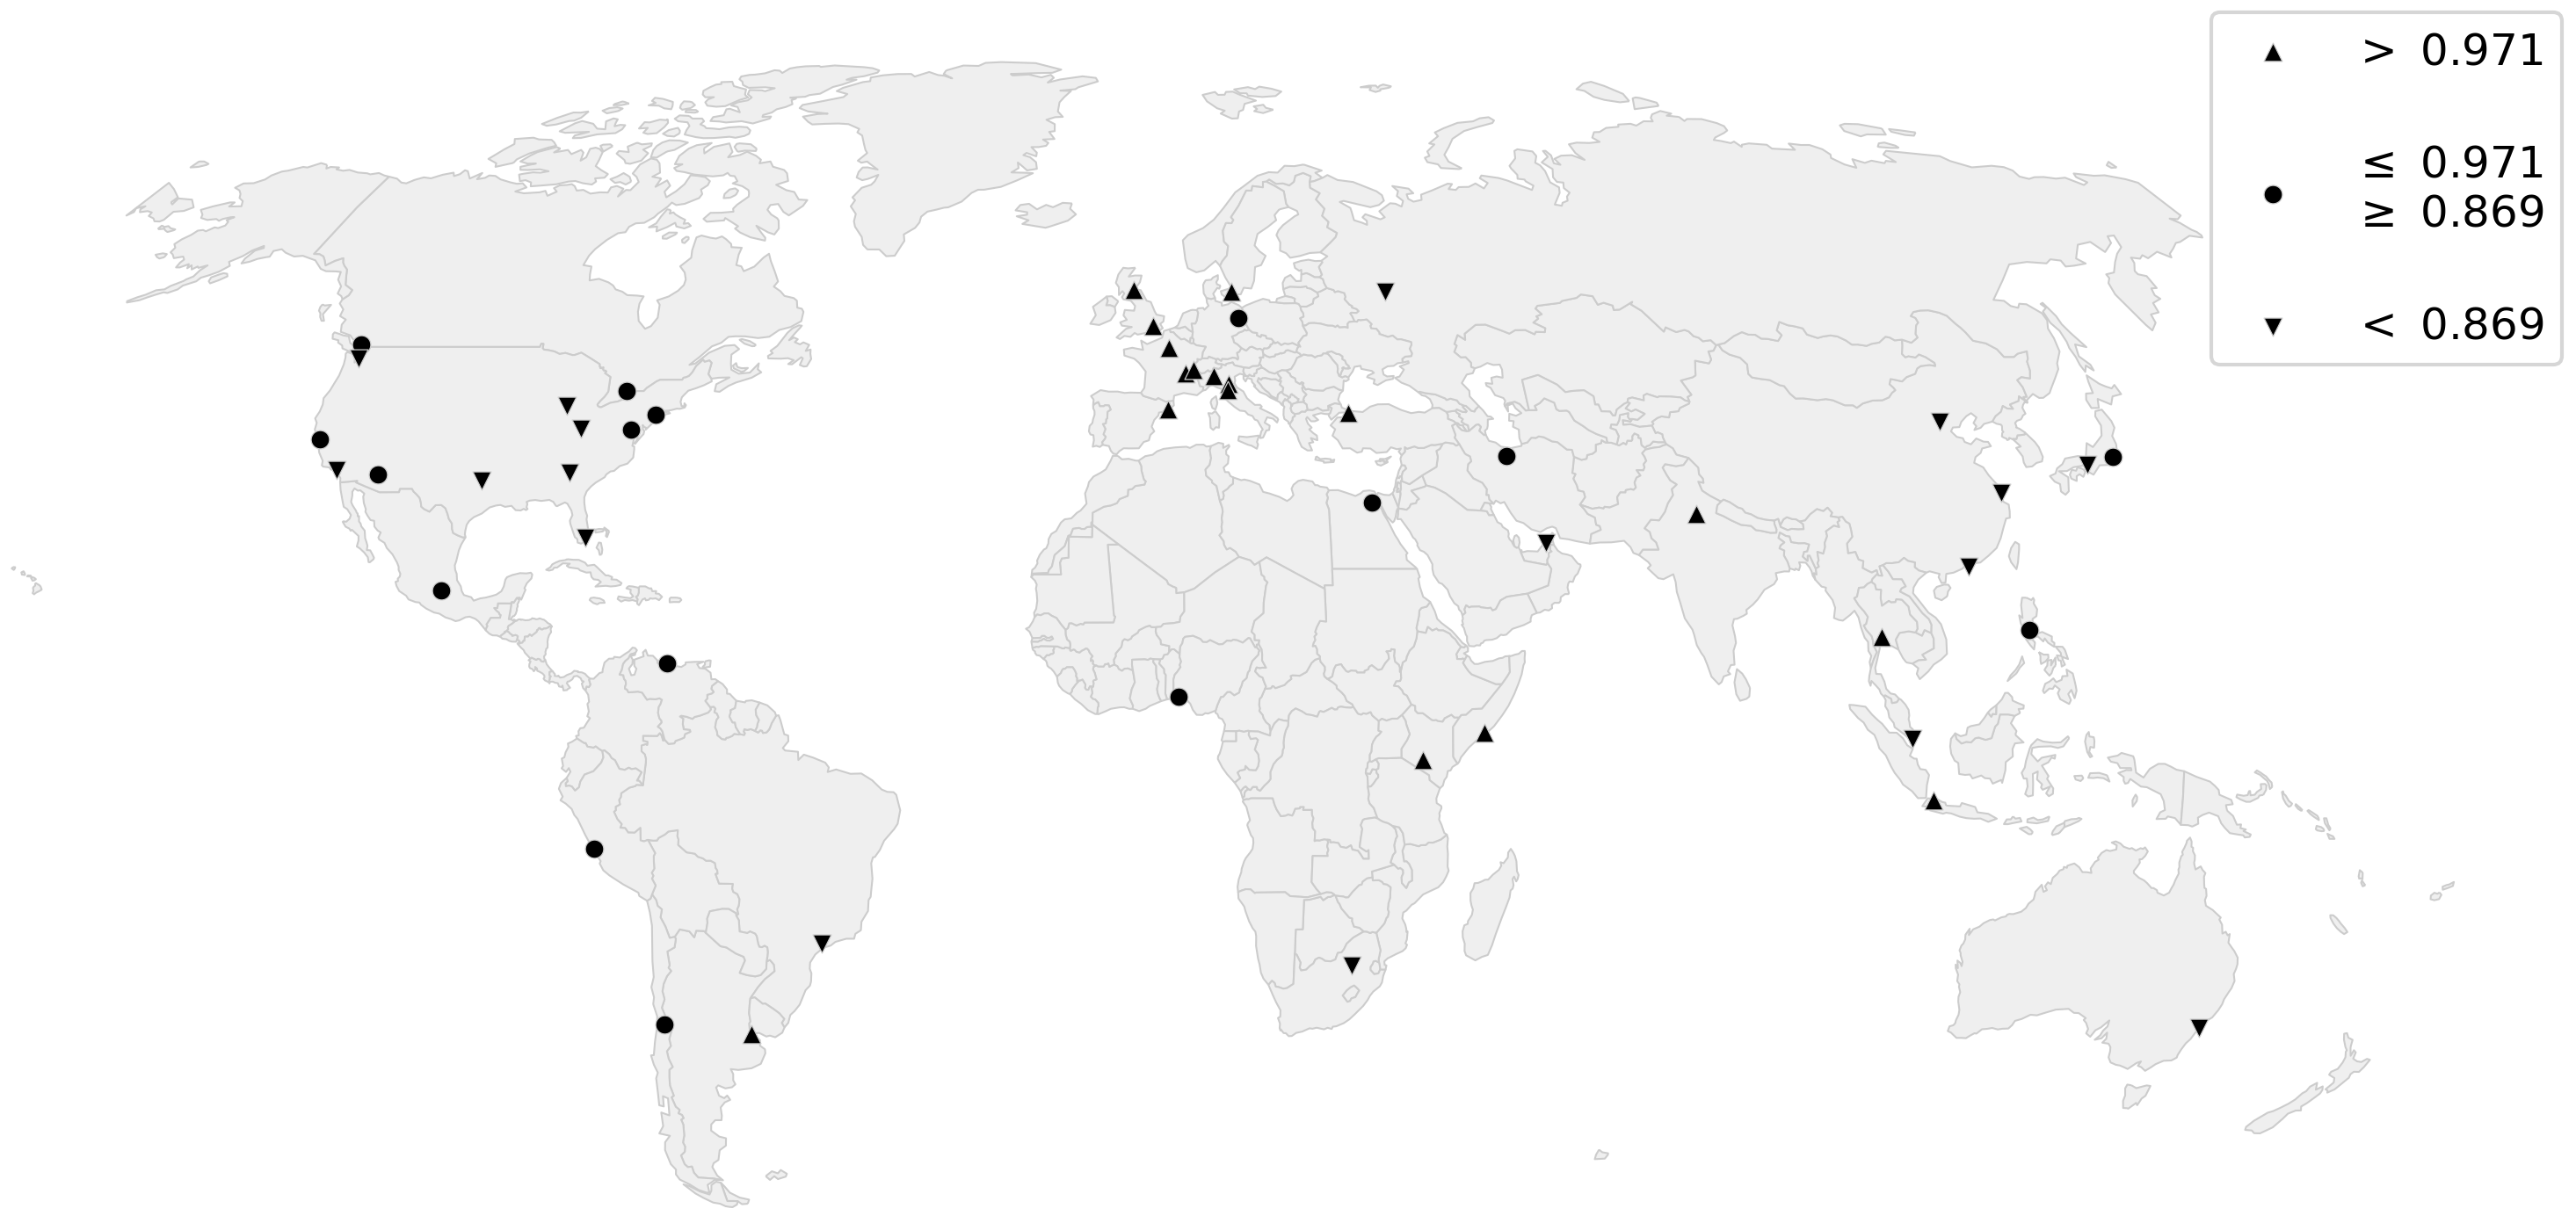
\includegraphics[width=0.95\textwidth]{fig_example.png}
    \caption{This is the caption of my figure.}\label{fig:world_map}
\end{figure*}

\subsection{Finding Two}

Present the details of your second finding here. Add figures and tables as needed. For example, see \autoref{tab:my_table}.

\begin{table*}[tbhp]
    \centering
    \caption{This is the caption of my table.}\label{tab:my_table}
    \tabularnums{\small
    \begin{tabular}{rrrr}
        \toprule
        Residential Pop &  Daytime Pop &  Land Area (km\textsuperscript{2}) &  Daytime Density \\
        \midrule
        1783  & 70,728 & 0.556 & 127,198 \\
        6172  & 42,635 & 0.446 &  95,652 \\
        2734  &  8,006 & 0.092 &  86,882 \\
        1500  &  4,850 & 0.057 &  85,743 \\
        4307  & 19,051 & 0.240 &  79,424 \\
        \bottomrule
    \end{tabular}}
\end{table*}

\section{Discussion}

Discussion: answer your question, advance your argument, and demonstrate significance. Return to research question and interpret (don't repeat) your findings as evidence for/against it. Tell a story: link your findings together to persuasively advance your argument. Significance: discuss specific implications for research and practice (the \enquote{so what}). Acknowledge study's limitations and alternative interpretations of your evidence: what opportunities are there for future research?

In general, people struggle most with writing an effective introduction and discussion. Perversely, these are also the most critical sections of your paper for persuading your readers (including peer reviewers).

\section{Conclusion}

Conclusion: succinctly wrap-up in one or two paragraphs. Summarize your topic, question, and argument. Summarize what you did, what you found, what it means, and why it matters.

Sometimes the introduction and background are merged into a single section. Sometimes the discussion and conclusion are merged into a single section. But this is the basic structure of an effective paper, be it a technical report or a scholarly article. The structure represents a loose symmetry. The introduction and conclusion roughly mirror each other by explaining the topic's importance, the research question, how you answered it and what you found, and its meaning/significance in the real world. The background and discussion roughly mirror each other by explaining what is known about the topic before (to motivate your specific study) and after your study (to advance our knowledge and impact the real world). The methods and findings sections roughly mirror each other by laying out what you did and then presenting what you found when you did so.

\section*{Acknowledgments}

The author wishes to thank the following people for their comments and support.

% print the footnotes as endnotes, if any exist
\IfFileExists{\jobname.ent}{\theendnotes}{}

% print the bibliography
\setlength{\bibsep}{0.00cm plus 0.05cm} % no space between items
\bibliographystyle{apalike}
\bibliography{references}

\end{document}
